  \subsection{Análisis de una señal modulada en frecuencia}

    Se procede a analizar una FM. Para ello se hace lo siguiente:

      \begin{figure}[H]
        \centering
          \frame{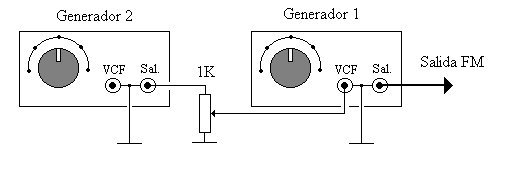
\includegraphics[width=0.8\textwidth]{Imagenes/ActividadPractica/6AnalisisDeUnaSeñalDeFM/EsquemaConexionGeneradores.png}}
          \caption{Conexión de los generadores.}
          \label{fig:Exp6EsquemaGeneradores}
      \end{figure}

    Inicialmente se procede a calibrar los generadores.

      \begin{figure}[H]
        \centering
        \begin{subfigure}[H]{0.48\textwidth}
          \frame{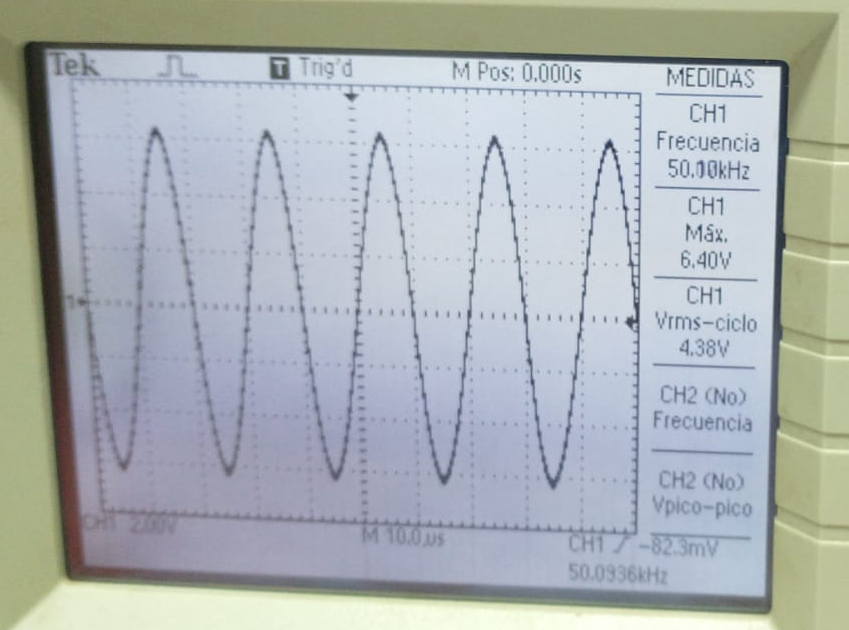
\includegraphics[width=\textwidth]{Imagenes/ActividadPractica/6AnalisisDeUnaSeñalDeFM/Exp6_Calibracion_G1.png}}
          \caption{Calibración G1.}
          \label{fig:Exp6CalibracionG1}
        \end{subfigure}
        \hfill 
        \begin{subfigure}[H]{0.48\textwidth}
          \frame{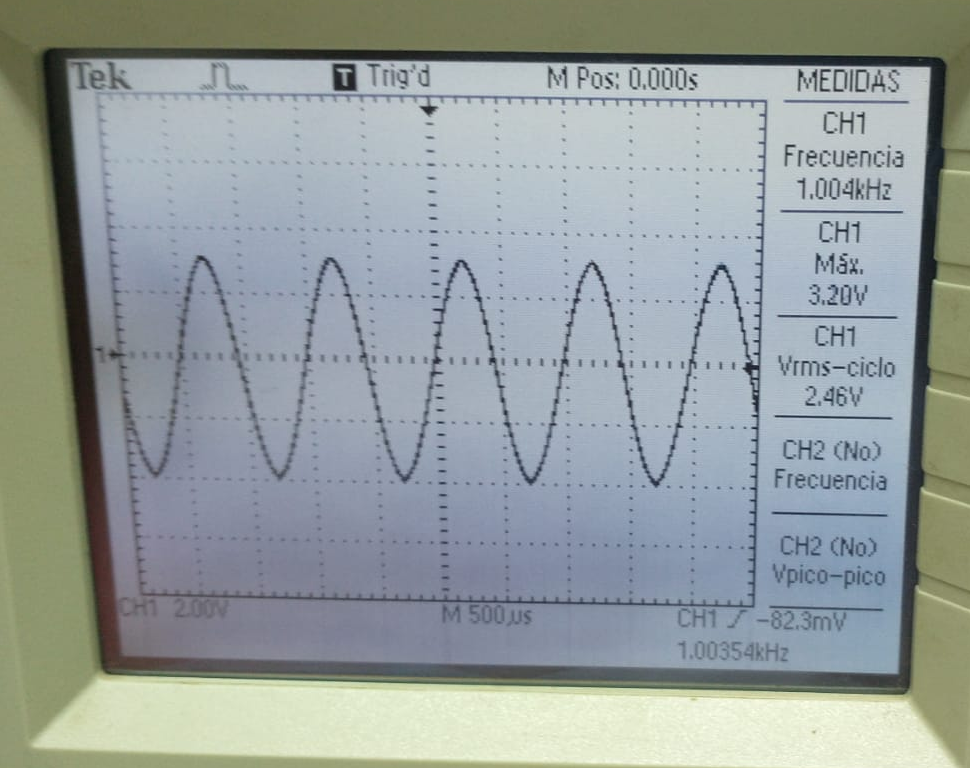
\includegraphics[width=\textwidth]{Imagenes/ActividadPractica/6AnalisisDeUnaSeñalDeFM/Exp6_Calibración_G2.png}}
          \caption{Calibración G2.}
          \label{fig:Exp6CalibracionG2}
        \end{subfigure}
      \end{figure}

    Se observa la señal a 1 ms por div.

      \begin{figure}[H]
        \centering
          \frame{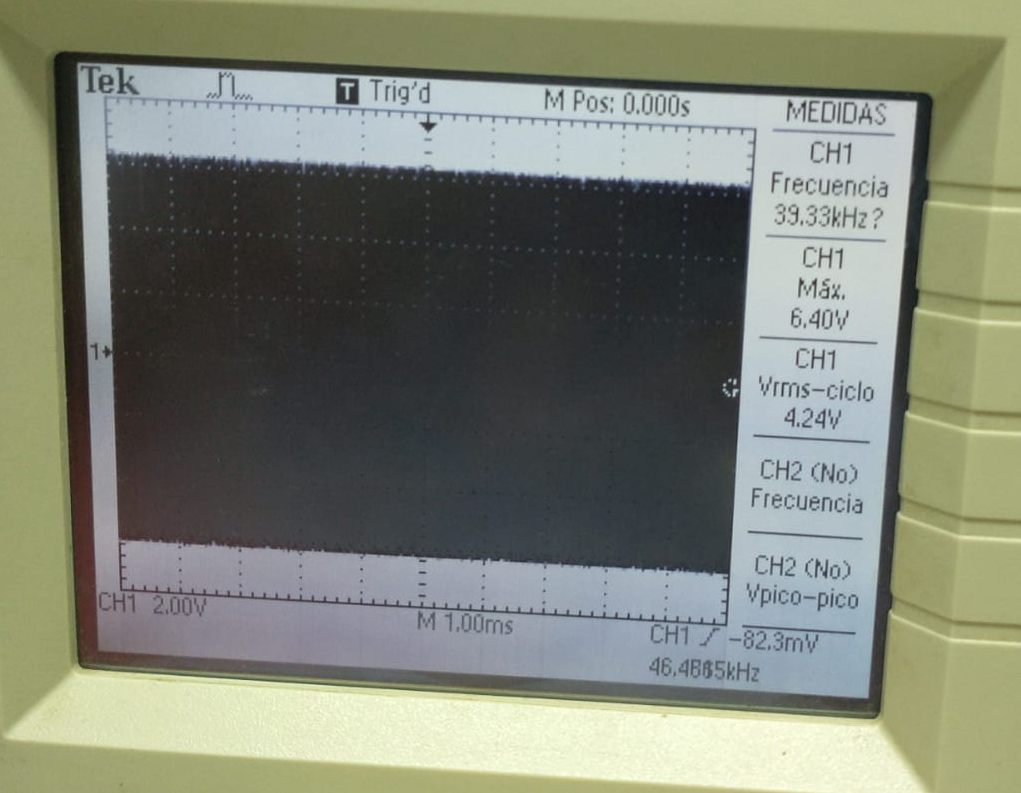
\includegraphics[width=0.5\textwidth]{Imagenes/ActividadPractica/6AnalisisDeUnaSeñalDeFM/Exp6_SeñalDeSalidaCon1msPorDiv.png}}
          \caption{1ms.}
          \label{fig:Exp6SeñalFM1ms}
      \end{figure}

    La salida FM en frecuencia configurada con adquisión promedio y normal 
    se ve.

      \begin{figure}[H]
        \centering
        \begin{subfigure}[H]{0.48\textwidth}
          \frame{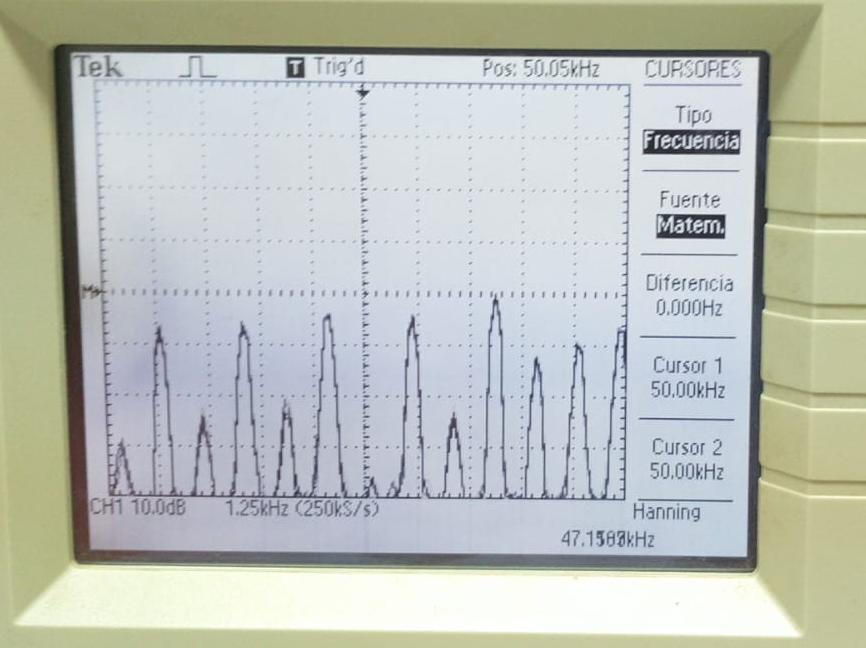
\includegraphics[width=\textwidth]{Imagenes/ActividadPractica/6AnalisisDeUnaSeñalDeFM/Exp6_SalidaFMEnFrecuenciaConfigurada.png}}
          \caption{FM con promedios.}
          \label{fig:Exp6SeñalFM}
        \end{subfigure}
        \hfill 
        \begin{subfigure}[H]{0.48\textwidth}
          \frame{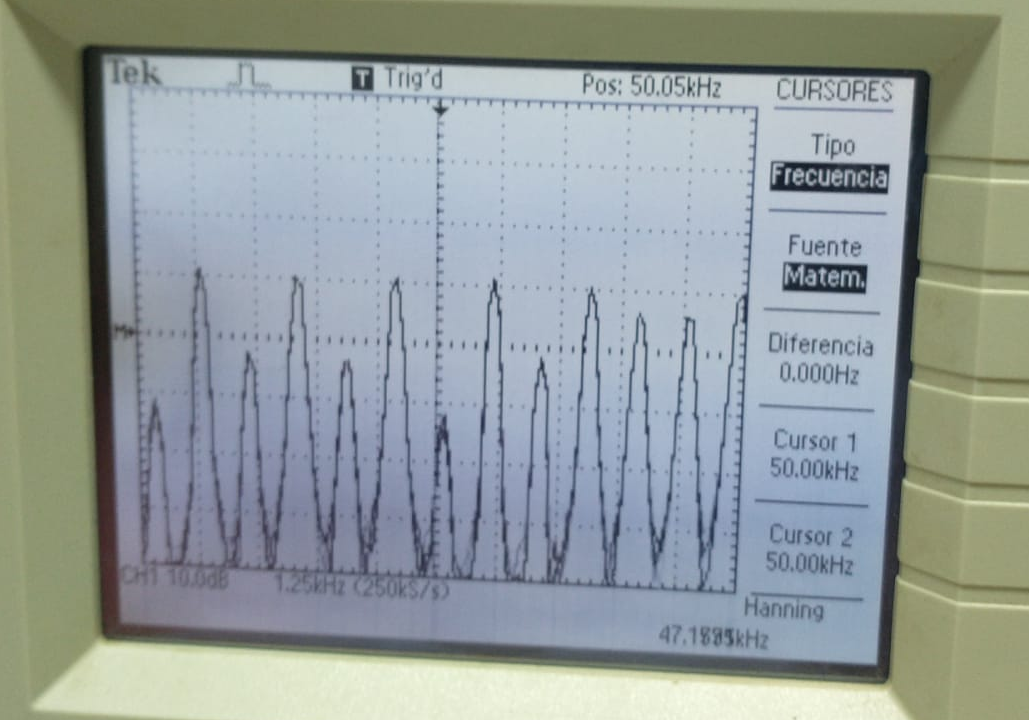
\includegraphics[width=\textwidth]{Imagenes/ActividadPractica/6AnalisisDeUnaSeñalDeFM/Exp6_SalidaFMEnFrecuenciaAdqNormal.png}}
          \caption{Adquisicion normal.}
          \label{fig:Exp6SeñalFMAdquisicionNormal}
        \end{subfigure}
      \end{figure}

    Se busca índice de modulación de 2.4, con promedios y sin promedios.

      \begin{figure}[H]
        \centering
        \begin{subfigure}[H]{0.48\textwidth}
          \frame{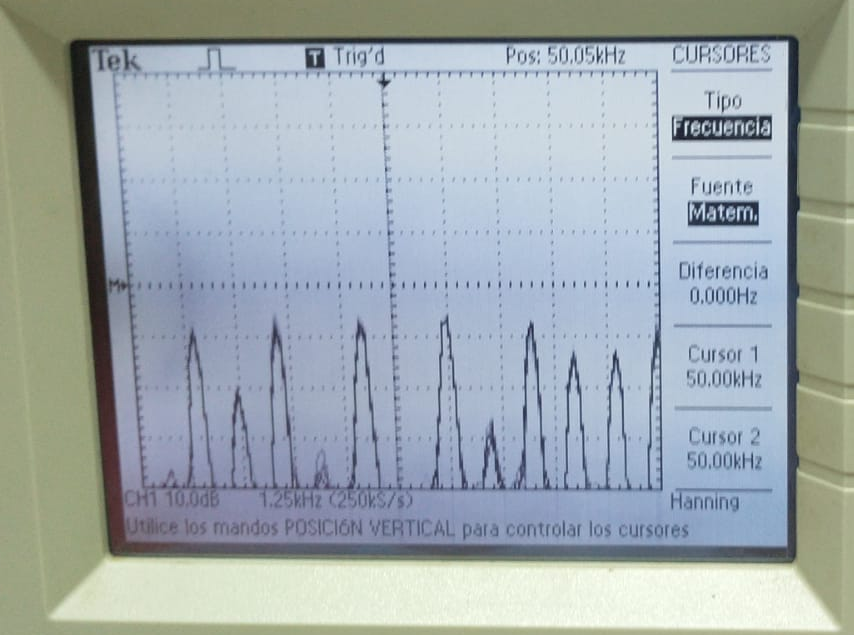
\includegraphics[width=\textwidth]{Imagenes/ActividadPractica/6AnalisisDeUnaSeñalDeFM/Exp6_SalidaFMconindice2_4yPromedios.png}}
          \caption{FM con promedios.}
          \label{fig:Exp6SeñalFMIndice2_4}
        \end{subfigure}
        \hfill 
        \begin{subfigure}[H]{0.48\textwidth}
          \frame{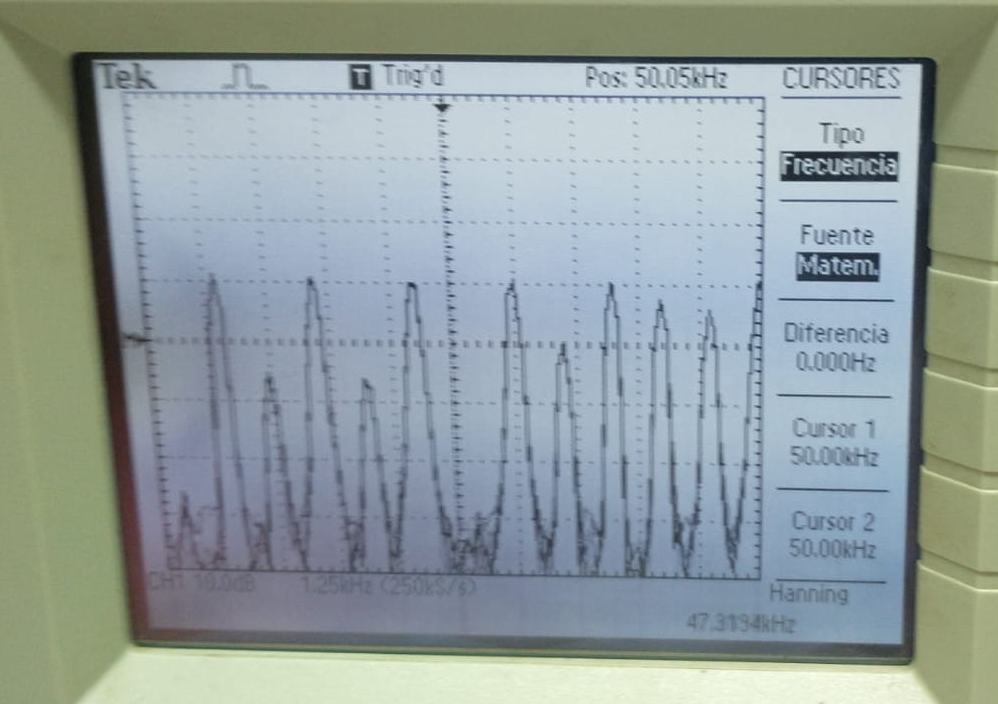
\includegraphics[width=\textwidth]{Imagenes/ActividadPractica/6AnalisisDeUnaSeñalDeFM/Exp6_SalidaFMindice2_4SinPromedios2.png}}
          \caption{Adquisicion normal.}
          \label{fig:Exp6SeñalFMIndice2_4AdquisicionNormal}
        \end{subfigure}
      \end{figure}   

    Se disminuye ligeramente el indice de modulación.

      \begin{figure}[H]
        \centering
          \frame{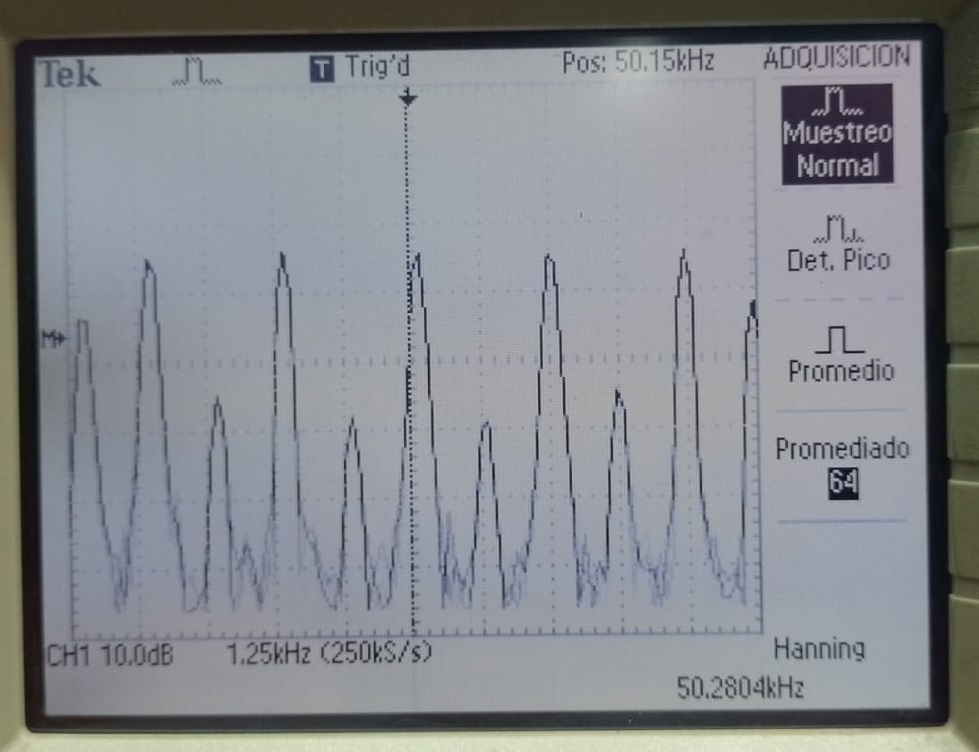
\includegraphics[width=0.5\textwidth]{Imagenes/ActividadPractica/6AnalisisDeUnaSeñalDeFM/Exp6_SalidaFMindiceligeramentedisminuido.png}}
          \caption{Índice ligeramente disminuído.}
          \label{fig:Exp6SeñalFMIndiceDisminuido}
      \end{figure}
    
    Se inyecta una señal cuadrada y se ven distintas ventanas.

      \begin{figure}[H]
        \centering
        \begin{subfigure}[H]{0.48\textwidth}
          \frame{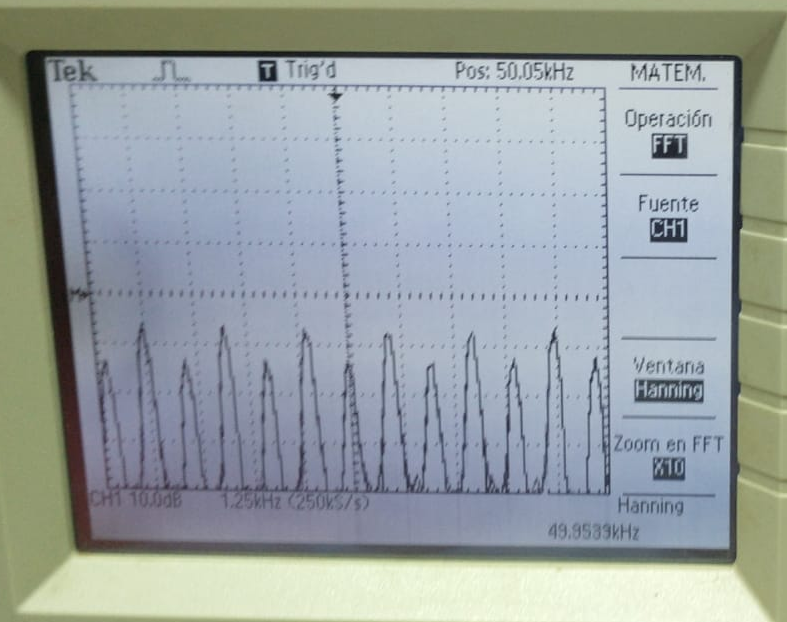
\includegraphics[width=\textwidth]{Imagenes/ActividadPractica/6AnalisisDeUnaSeñalDeFM/Exp6_SeñalFMConmodulanteCuadradaSinPromedios.png}}
          \caption{Señal cuadrada con ventana Hanning.}
          \label{fig:Exp6SeñalFMModulanteCuadradaHanning}
        \end{subfigure}
        \hfill 
        \begin{subfigure}[H]{0.48\textwidth}
          \frame{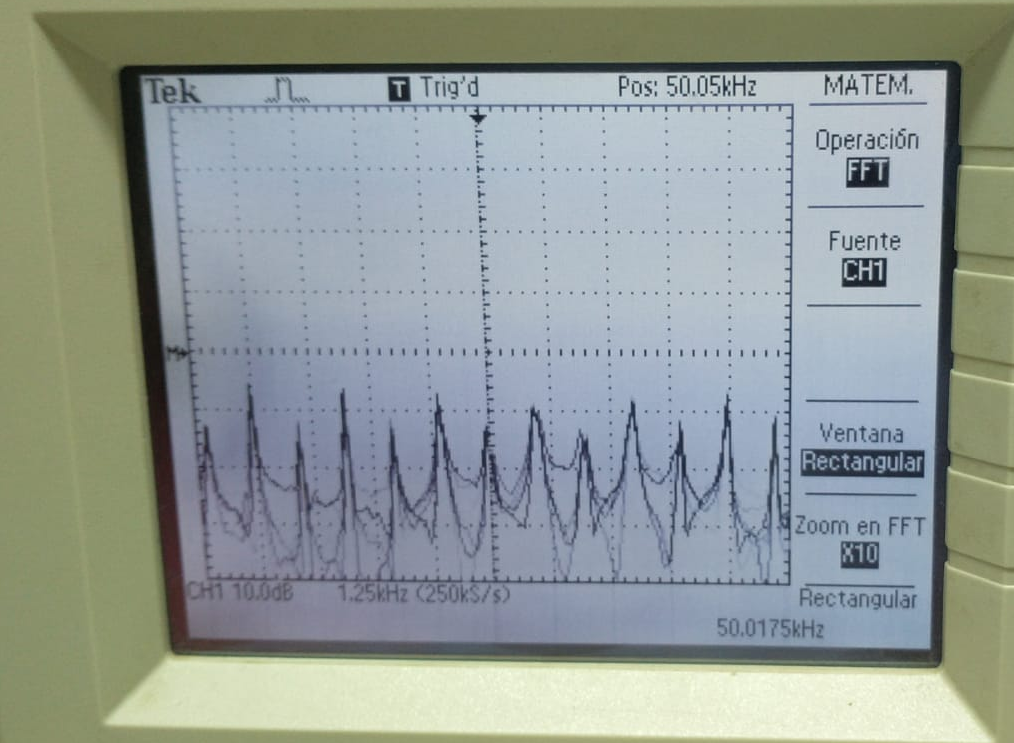
\includegraphics[width=\textwidth]{Imagenes/ActividadPractica/6AnalisisDeUnaSeñalDeFM/Exp6_SeñalFMConModulanteCuadradaSinPromediosVentanaHanning.png}}
          \caption{Señal cuadrada con ventana Rectangular.}
          \label{fig:Exp6SeñalFMModulanteCuadradaRectangular}
        \end{subfigure}
        \begin{subfigure}[H]{0.48\textwidth}
          \frame{
\includegraphics[width=\textwidth]{Imagenes/logo-utn.png}}
          \caption{Señal cuadrada con ventana Flattop.}
          \label{fig:Exp6SeñalFMModulanteCuadradaFlattop}
        \end{subfigure}
      \end{figure}   

      Se inyecta una señal triangular y se ven distintas ventanas.

      \begin{figure}[H]
        \centering
        \begin{subfigure}[H]{0.48\textwidth}
          \frame{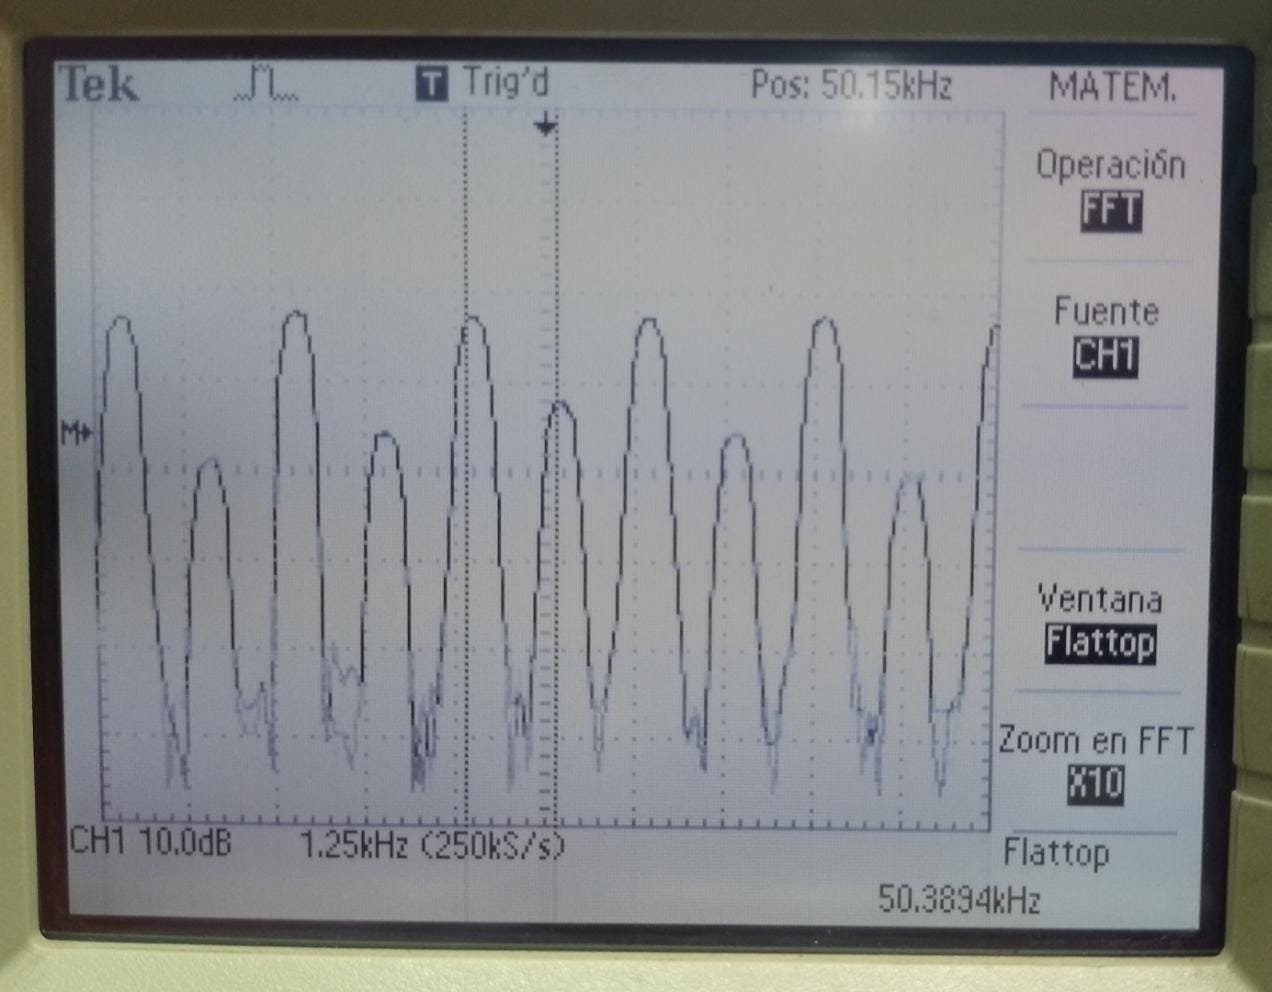
\includegraphics[width=\textwidth]{Imagenes/ActividadPractica/6AnalisisDeUnaSeñalDeFM/Exp6_SeñalFMConModulanteTriángularVentanaFlattop.png}}
          \caption{Señal triangular con ventana Hanning.}
          \label{fig:Exp6SeñalFMModulanteTriangularHanning}
        \end{subfigure}
        \hfill 
        \begin{subfigure}[H]{0.48\textwidth}
          \frame{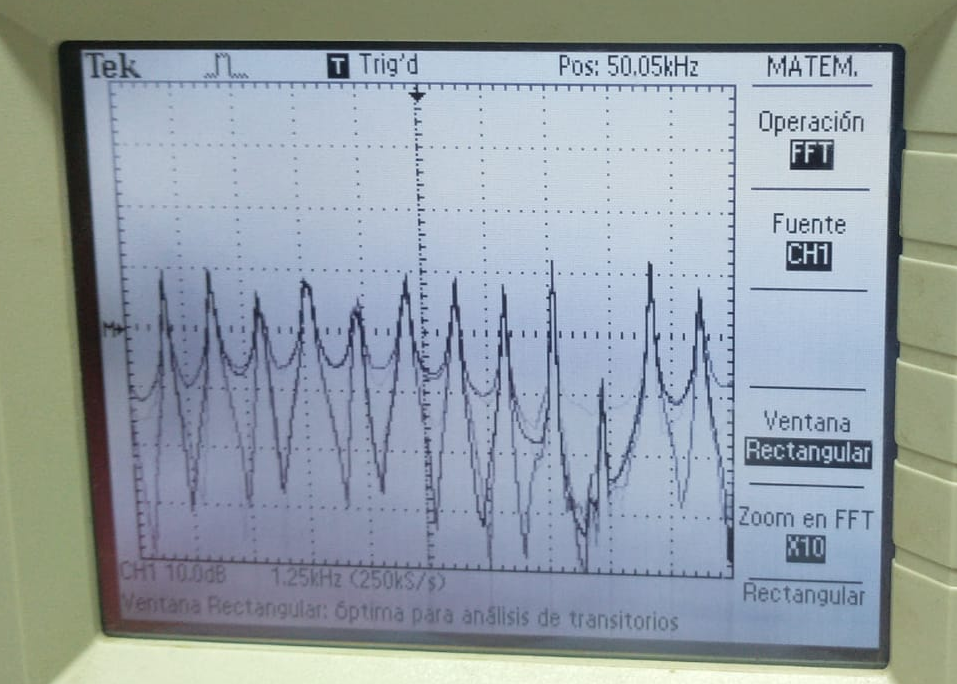
\includegraphics[width=\textwidth]{Imagenes/ActividadPractica/6AnalisisDeUnaSeñalDeFM/Exp6_SeñalFMConmodulanteTriángularSinPromedioVentanaRectangula.png}}
          \caption{Señal triangular con ventana Rectangular.}
          \label{fig:Exp6SeñalFMModulanteTriangularRectangular}
        \end{subfigure}
       \begin{subfigure}[H]{0.48\textwidth}
          \frame{
\includegraphics[width=\textwidth]{Imagenes/logo-utn.png}}
          \caption{Señal triangular con ventana Flattop.}
          \label{fig:Exp6SeñalFMModulanteTriangularFlattop}
        \end{subfigure}
      \end{figure}         

    Se mide la frecuencia de las bandas laterales.

      \begin{figure}[H]
        \centering
        \begin{subfigure}[H]{0.48\textwidth}
          \frame{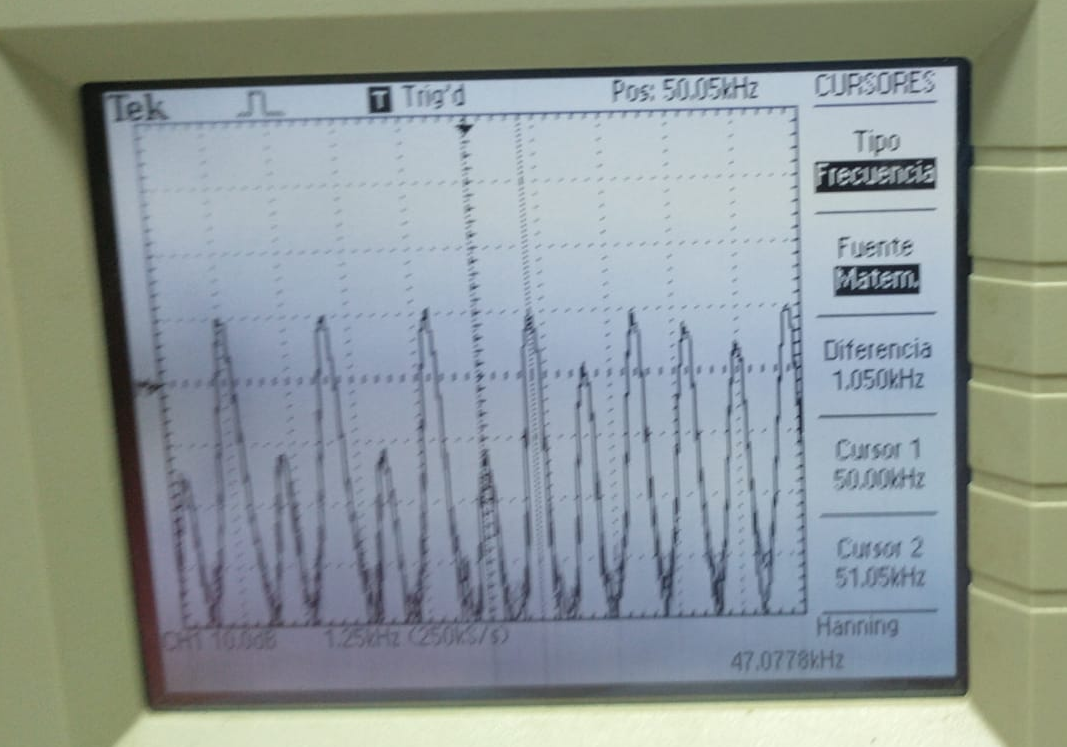
\includegraphics[width=\textwidth]{Imagenes/ActividadPractica/6AnalisisDeUnaSeñalDeFM/Exp6_SeñalFMMedicionDeFrecModulante_DiferenciaEntrePortadoraYBandaLateralIzq.png}}
          \caption{Diferencia con banda lateral izquierda.}
          \label{fig:Exp6SeñalFMDifBandaLateralIzq}
        \end{subfigure}
        \hfill 
        \begin{subfigure}[H]{0.48\textwidth}
          \frame{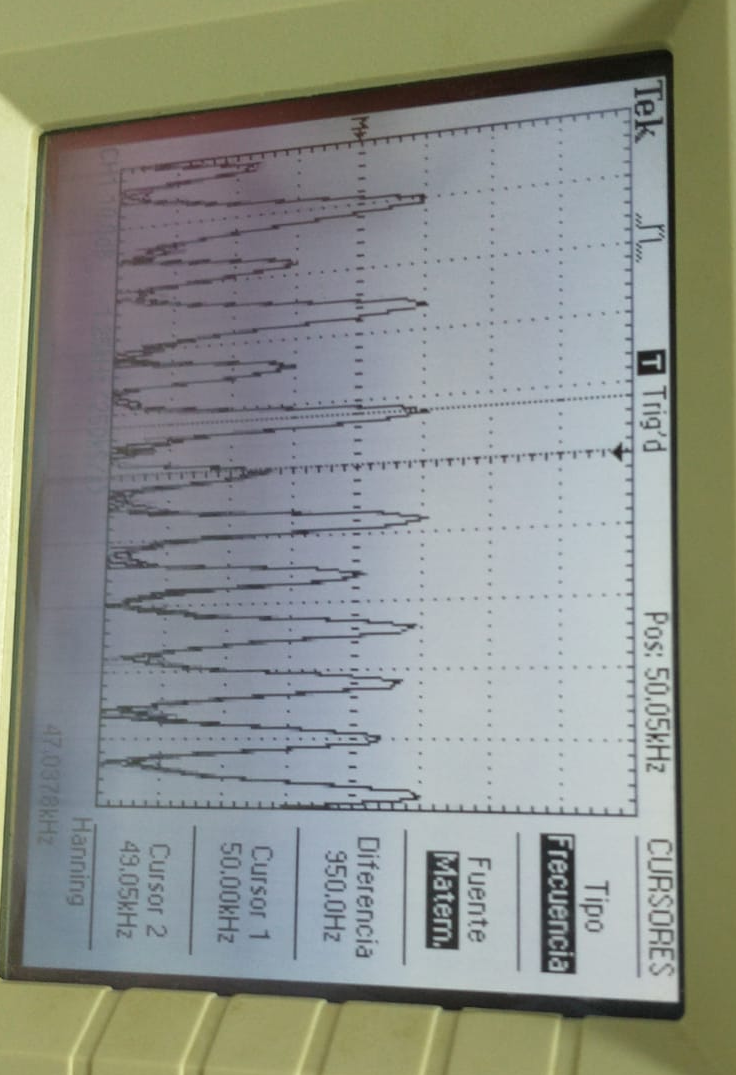
\includegraphics[width=\textwidth]{Imagenes/ActividadPractica/6AnalisisDeUnaSeñalDeFM/Exp6_SeñalFMMedicionDeFrecModulante_DiferenciaEntrePortadoraYBandaLateralDer.png}}
          \caption{Diferencia con banda lateral derecha.}
          \label{fig:Exp6SeñalFMDifBandaLateralDer}
        \end{subfigure}
      \end{figure}  
    